\section{Ristrutturazione schema E-R}
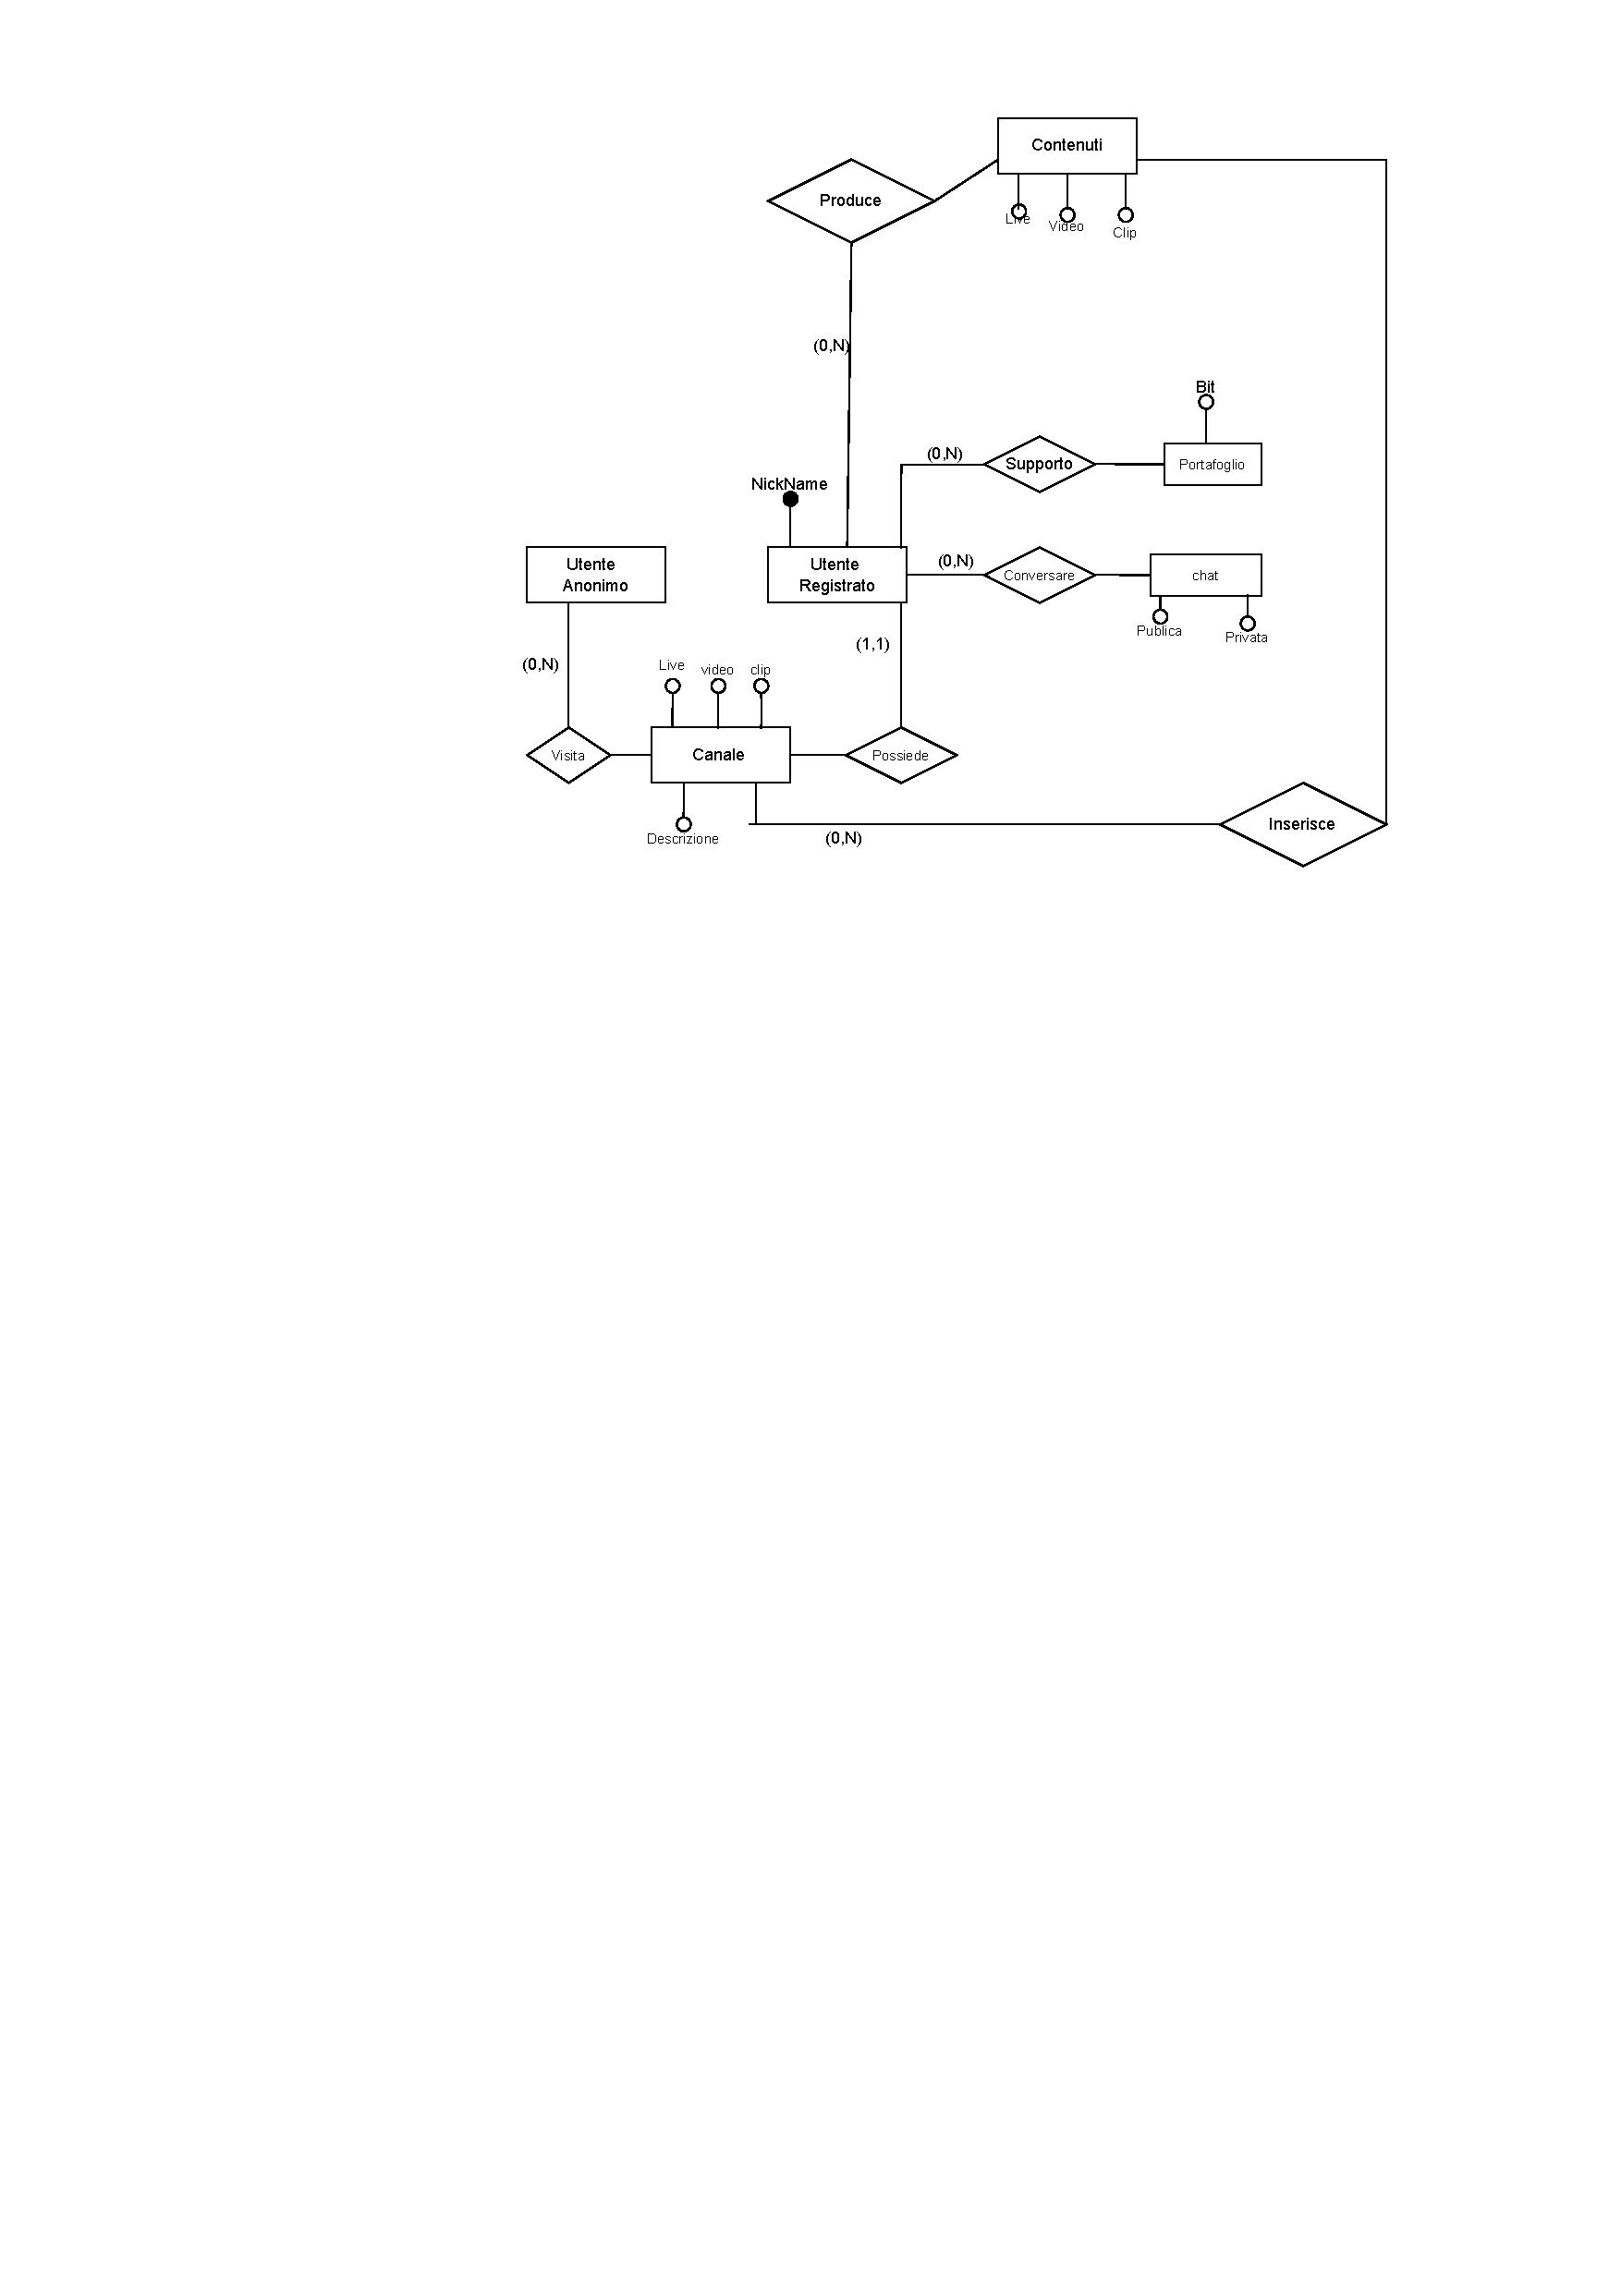
\includegraphics[width=\textwidth]{resources/e_r_ridotto.pdf}


\subsection{Business rules E-R ristrutturato }
\begin{itemize}
    \item Gli attributi live ,video ,clip presenti nell'entità \textbf{canale} indicato un oggetto finito e caricato al suo interno.
    \item Gli attributi live ,vide ,clip presenti sull'entitá \textbf{contenuti} indicano un oggetto che ancora o è in fase di produzione o è un prodotto finito ma non caricato sul canale del proprietario. 
    \item Gli utenti anonimi non possono supportare gli streamer. 
    \item Gli streamer sono utenti registrati che caricano  o trasmettono contenuti. 
    \item Ogni utente registrato ha un nickname. 
    \item Il nickname scelto dall'utente registrato sarà anche il nome del canale. 
    \item Ogni canale ha una Descrizione. 
    \item Le live sono contenuti o in tempo reale.
    \item I video sono live già concluse. 
    \item Le clip sono brevi estratti di video. 
    \item Un utente anonimo non può conversare con altri utenti.
    \item Un utente anonimo non possiede un canale. 
\end{itemize}
